% This is samplepaper.tex, a sample chapter demonstrating the
% LLNCS macro package for Springer Computer Science proceedings;
% Version 2.21 of 2022/01/12
%
\documentclass[runningheads]{llncs}
%
\usepackage[T1]{fontenc}
% T1 fonts will be used to generate the final print and online PDFs,
% so please use T1 fonts in your manuscript whenever possible.
% Other font encondings may result in incorrect characters.
%
\usepackage{amsmath}
\usepackage{graphicx}
% Used for displaying a sample figure. If possible, figure files should
% be included in EPS format.
%
% If you use the hyperref package, please uncomment the following two lines
% to display URLs in blue roman font according to Springer's eBook style:
%\usepackage{color}
%\renewcommand\UrlFont{\color{blue}\rmfamily}
%
\begin{document}
%
\title{Automatic Knowledge Acquisition System with Large Language Model in Academic Domain}
%
%\titlerunning{Abbreviated paper title}
% If the paper title is too long for the running head, you can set
% an abbreviated paper title here
%
\author{Ahmad Julius Tarigan\inst{1}\orcidID{0009-0000-0369-5782} \and
Kemas Rahmat Saleh Wiharja, Ph.D\inst{1}\orcidID{0000-0002-3660-8128} \and
Dade Nurjanah, Ph.D\inst{1}\orcidID{0000-0001-9318-8409}}
%
\authorrunning{A. J. Tarigan et al.}
% First names are abbreviated in the running head.
% If there are more than two authors, 'et al.' is used.
%
\institute{School of Computing, Telkom University, Bandung, Indonesia \\
\email{juliusahmad@student.telkomuniversity.ac.id} \\
\email{bagindokemas@telkomuniversity.ac.id} \\
\email{dadenurjanah@telkomuniversity.ac.id}}
%
\maketitle              % typeset the header of the contribution
%
\begin{abstract}
In academic, a significant challenge in knowledge acquisition involves combining explicit information from academic documents and implicit knowledge through interviews with experts, such as program secretaries, and lecturers. This research proposes an automated Knowledge Acquisition System that utilizes the Large Language Models to address inefficiencies in explicit and implicit knowledge extraction. The background of the research highlights the urgency of efficiency in knowledge acquisition to support academic processes, including problems involving final assignments, graduation information, practical work, and course registration. Traditional methods tend to be less effective in capturing explicit knowledge, hindering a holistic understanding of the academic domain. This research integrates Large Language Models to collect explicit knowledge from documents and implicit knowledge from interviews, creating a system architecture that facilitates comprehensive knowledge acquisition. Key results demonstrate the system's effectiveness in knowledge acquisition, with the potential to improve various academic processes, including Final Project completion, Practical Work, Graduation, Course Registration, and External Activities. This research achieves significant advances in knowledge acquisition methodologies in academic environments, offering a holistic and efficient approach to managing explicit and implicit knowledge, while providing solutions to a number of academic problems.

\keywords{knowledge acquisition \and large language model \and academic domain \and explicit knowledge \and implicit knowledge.}
\end{abstract}
%
%
%
\section{Introduction}
\subsection{Background}

The focus of this research is the development of the Knowledge Acquisition System (KAS) for the academic domain utilizing Large Language Models (LLMs). Success in higher education largely depends on students' understanding of various academic processes, such as final projects, graduation information, internship placements, and course registrations. Unfortunately, at any university in Indonesia, this information is often extensive and complex, leading to diverse interpretations. Knowledge regarding these aspects is frequently implicit, known only to faculty or other academic staff. Therefore, there is a need to extract both explicit and implicit knowledge. In this context, developing the KAS using LLMs becomes crucial to address bias issues and ensure more consistent and accurate information retrieval.

The background of this research stems from the imperfections in current knowledge acquisition practices. Traditional methods often fail to capture the implicit knowledge hidden within academic documents, resulting in incomplete understanding. In knowledge management, the term "implicit" refers to tacit knowledge that is not clearly articulated in written or formal forms.

For instance, consider the guidelines for final projects. Although there are official guidelines provided by the academic institution, interpretations of these guidelines may vary among faculty and students. Some aspects might not be explicitly documented in the guidelines, and tacit knowledge from experts can help standardize perceptions and clarify interpretations that may otherwise lead to discrepancies.

The choice of LLMs as the language model for the KAS is based on their ability to handle knowledge extraction from human language. This approach is expected to address challenges in understanding and aligning complex information, thereby fulfilling broader informational needs within the academic realm.

Thus, leveraging LLMs in KAS can help overcome various challenges in knowledge acquisition within academic environments. This system aims to enhance the accuracy and completeness of obtained information, ensuring that hidden knowledge can be accessed and utilized effectively, thereby supporting better knowledge management in the academic domain.

\subsection{Problem Statement}
This research focuses on developing the KAS in the academic domain using LLMs. To facilitate interaction with the LLMs, we utilize the Langchain framework, a tool designed to integrate and optimize the use of language models in specific applications. The gaps identified in the current knowledge acquisition conditions within academic environments include several critical aspects affecting efficiency and depth of understanding:
\begin{enumerate}
    \item \textbf{Difficulty in Extracting Implicit Knowledge} \\
    Traditional methods often fail to capture implicit knowledge in academic documents due to the time-consuming and error-prone nature of manual processes. Manual data extraction typically involves sifting through large volumes of academic documents, which can lead to missed information and inconsistent results \cite{kiran2019}. This inefficiency underscores the need for automated systems like KAS, which can leverage LLMs to accelerate and improve the accuracy of information extraction.
    
    \item \textbf{Collection and Understanding of Tacit Knowledge} \\
    Tacit knowledge, often held by academic secretaries and faculty, is difficult to capture and document. This is due to the high level of busyness of the study program secretary and lecturers, which means that it takes a long time to structure and write down their tacit knowledge. The KAS with LLMs and interview techniques can identify, codify, and integrate this tacit knowledge, making it more accessible.
    
    \item \textbf{Limitations of Traditional Methods in Aligning Information} \\
    Relevant information in academic context is scattered across various documents and individuals, leading to varying interpretations. The KAS using LLMs can automatically consolidate and align knowledge from diverse sources, ensuring that the information produced is comprehensive and well-structured.
    
    \item \textbf{Need for an Adaptive and Responsive System} \\
    The dynamic nature of academic environments requires a system that is flexible and can be updated regularly. KAS developed with LLMs technology such as Langchain can be adapted to accommodate changes in policies, procedures, and new knowledge, ensuring the system remains relevant and effective \cite{deepLearning2023LangChain}.
\end{enumerate}

By addressing these gaps, this research aims to contribute significantly to enhance the efficiency and depth of understanding in the academic domain. The development of the KAS utilizing LLMs could serve as an innovative solution to improve knowledge acquisition processes, ensuring that important and relevant information is easily accessible to all involved parties.

\subsection{Objective}
The objective of this research is to develop the KAS for the academic domain using OpenAI's language model, GPT-3.5. The primary goals are to create an effective KAS capable of collecting explicit knowledge from academic documents and extracting tacit knowledge through interviews with experts, such as academic secretaries and faculty members. Additionally, this research aims to enhance the accuracy of knowledge extraction from these sources by focusing on identifying and addressing potential barriers or noise, resulting in cleaner and more reliable data. Another goal is to efficiently integrate explicit knowledge from academic documents with tacit knowledge from interviews. This integration is expected to form a more holistic and in-depth understanding of the academic domain, creating a more complete and accurate representation.

In the development phase of the KAS, this research also aims to establish evaluation metrics that effectively measure the system's performance. These metrics will include accuracy in capturing knowledge, processing speed, and adaptability to various types of documents and interview contexts. Finally, the research seeks to identify the contributions of the KAS to overall academic management. By detailing its potential contributions, it is hoped that the KAS will positively impact decision-making efficiency, curriculum planning, and human resource management in the academic context. By achieving these objectives, the research aims to provide a significant contribution to the advancement of KAS in the academic context, opening opportunities for improved academic management processes overall.

\section{Literature Review}
\subsection{Knowledge Management}
Knowledge integration is a combination of social skills and cooperation. It is the process of exchanging ideas between individuals and organizations \cite{Gao2021}. Knowledge management is well suited to the need for clear reporting and transparency for public administration \cite{Bem2022}.Tacit knowledge and explicit knowledge are two fundamental categories in the study of knowledge management. Tacit knowledge refers to the nuanced and often unspoken insights that arise from personal experiences, intuitions, and reflections. It is inherently unstructured and challenging to document, residing deeply within individuals and often revealed through practice and interaction. In contrast, explicit knowledge is systematically articulated and documented, encompassing data, information, and formal documents that can be easily communicated, shared, and stored. Explicit knowledge is structured and can be readily accessed, analyzed, and utilized by others. The interplay between these types of knowledge is crucial for effective knowledge management and organizational learning \cite{vincent2022}. 

\subsection{Knowledge Acquisition System}
The study of knowledge representation forms a critical foundation for developing effective and efficient KAS. One of the most recent and popular representation of knowledge is graph. Recent research by Hogan et al. \cite{Hogan2021} offers a comprehensive review of knowledge graphs, covering the challenges and lessons learned from their implementation at an industrial scale. This work is highly relevant for advancing KAS by providing insights into managing complex knowledge structures. 

Additionally, Noy et al. \cite{Noy2019} highlight the lessons and challenges involved in building industrial-scale knowledge graphs, offering valuable perspectives for developing systems that manage open web information more effectively. Paulheim \cite{Paulheim2017} also emphasizes the importance of refining knowledge graphs through various approaches and evaluation methods, contributing to the improvement of data quality. According to \cite{wiharja2020iterative}, a knowledge graph is a knowledge that is presented in triple format (entity as a subject, predicate, entity or literal as an object). By integrating these approaches, recent research indicates that graph-based knowledge representation and structured refinement methods can lead to more efficient and accurate systems for managing open web information.

In the context of this review, there is a significant shift towards utilizing LLMs in knowledge acquisition. One relevant study is the work detailing the use of LLMs in the development of KAS. The utilization of LLMs, as described by Brown \cite{Brown2020}, enables systems to understand and extract knowledge from documents with a higher level of linguistic complexity. The transition to LLMs was driven by the limitations of knowledge graphs, such as their reliance on structured data and the difficulty of capturing tacit knowledge, which often requires an understanding of nuanced context and language. LLMs, by contrast, excel at processing unstructured data and can capture both explicit and tacit knowledge, making them particularly effective for complex environments like academia, where knowledge is often context-dependent and dynamic.

The comparison between graph models and language models highlights the strengths of LLMs, particularly in handling unstructured data and understanding contextual nuances. LLMs like GPT provide holistic knowledge acquisition, addressing limitations in traditional knowledge extraction. In \cite{Krause2024}, discusses how Generative AI (GAI), such as ChatGPT, enhances learning efficiency and personalization in education but also raises concerns about academic integrity and reliance on technology. These insights further emphasize the flexibility of LLMs in KAS.

\subsection{Large Language Models}
LLMs are advanced language models trained using deep learning techniques on large text corpora. A notable example of LLMs is GPT (Generative Pre-trained Transformer) developed by OpenAI \cite{Brown2020}. LLMs possess the capacity to understand and generate text with high complexity. These models are typically trained on specific tasks, such as next-word prediction or context understanding, making them highly useful in various applications, including natural language processing, text generation, and even machine translation. In the context of knowledge acquisition, In the realm of knowledge systems, frameworks like LangChain enhance LLMs capabilities by providing essential tools to handle structured and unstructured data. LangChain bridges LLMs with Vector Stores, allowing seamless interaction between text data, embedding models, and memory structures, which is crucial for efficient long-term data storage and retrieval in dynamic applications \cite{deepLearning2023LangChain}. The integration of LangChain with LLMs like GPT has enabled advancements in document processing, question answering, and chatbot development by supporting large datasets and context-aware conversations. This combination fosters real-time interaction with diverse data types, creating highly scalable and responsive KAS.

\subsection{Vector Databases}
Vector databases represent a concept in database management that uses vectors or mathematical representations of data. This approach enables vector-based data search and analysis, providing the ability to evaluate similarities between data vectors. In natural language processing, vector databases can be used to find similarities between texts based on vector representations of words or phrases \cite{Manning2008}. This approach is often employed in applications such as document retrieval and text classification.

\subsection{ROUGE Score}
ROUGE (Recall-Oriented Understudy for Gisting Evaluation) is an automated evaluation metric used to assess the success of text summarization systems by comparing the generated summaries with reference texts. One commonly used ROUGE score is ROUGE-N, which measures the overlap of unigrams, bigrams, or other n-grams between the generated summary and the reference text \cite{Lin2004}. ROUGE, introduced by Lin \cite{Lin2004}, has become a standard method for evaluating summarization systems and continues to be used in natural language processing research. It provides a deeper understanding of how well the generated summaries align with reference texts considered as the gold standard.

\subsection{BERT Score}
Systems can also be evaluated using the LLMs itself. LLMs can assess answer relevance by considering semantic similarity between the generated answers and reference answers. This method employs techniques like BERTScore, proposed by Zhang et al. \cite{Zhang2020}, to evaluate contextual similarity using BERT embedding representations. Semantic evaluation ensures that the answers provided are not only factually correct but also relevant and contextually appropriate. Recent studies by Goyal et al. \cite{Goyal2020} emphasize the importance of semantic similarity evaluation to ensure that LLMs do not introduce bias or errors in their assessments. Thus, combining manual expert evaluation with semantic evaluation by the LLMs itself provides a comprehensive approach to assessing the accuracy and relevance of the answers generated by the system.

\subsection{Manual Evaluation}
Manual evaluation with expert assistance is a crucial method for assessing the accuracy and relevance of answers produced by the system. This approach involves domain experts providing assessments based on criteria such as accuracy, completeness, and coherence. In this study, manual evaluation is conducted through expert surveys to assess the relevance of answers from the developed LLMs model. This method is similar to approaches used in recent research on evaluating text generation, where structured questionnaires and expert judgments are utilized to obtain more reliable assessments. For example, Guo et al. \cite{Guo2024} discuss improving text generation for product descriptions through human behavioral evaluation, while Celikyilmaz et al. \cite{Celikyilmaz2020} provide a comprehensive survey on various evaluation methods for text generation. Experts provide feedback based on factual accuracy, completeness of information, and contextual appropriateness of the answers provided by the system.

\section{System}
The third part of this research discusses the proposed solution to address the knowledge acquisition problem in an academic environment. The proposed system is designed to automatically acquire knowledge by utilizing data from interviews with experts such as study program secretaries, and lecturers, as well as information contained in academic documents. 

\begin{figure}
    \centerline{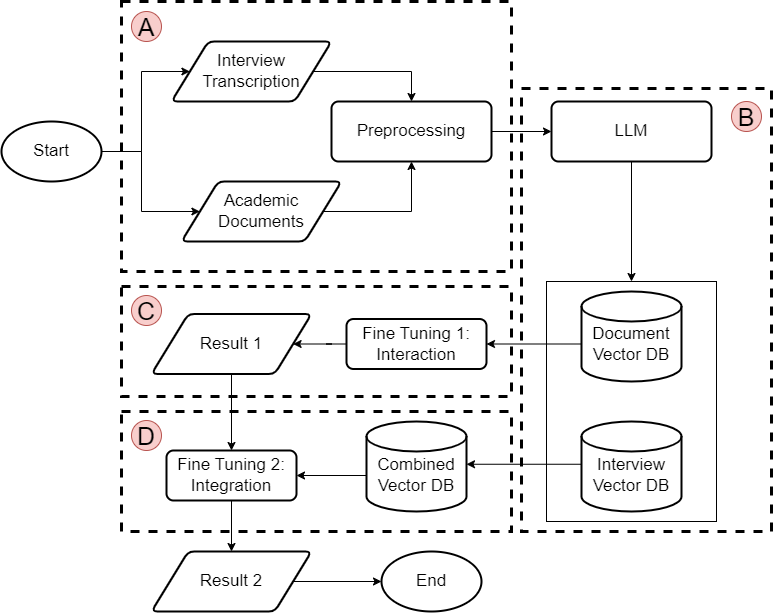
\includegraphics[scale=0.3]{eng-main.png}}
    \caption{System Flowchart}
    \label{fig:main-flowchart}
\end{figure}

The process broadly starts with reading and collecting data from interviews and documents, followed by a preprocessing step to prepare the data. The next step involves a LLMs to understand the content and generate a vector representation of the collected information. 

Then, the vector representation is then stored into a Vector Database (Vector DB) which will be the source of knowledge. The system involves two stages of fine-tuning, first process begins with documents only, where the system extracts relevant information from academic documents and generates \textbf{Result 1}, an answer based solely on the document dataset. In the second stage, the system combines information from multiple sources, such as interviews and documents, during a broader fine-tuning process. This produces \textbf{Result 2}, an answer generated by integrating knowledge from both documents and interviews, offering more comprehensive and contextualized responses. The flow of this process is illustrated in Figure \ref{fig:main-flowchart}.

The development of the system involves the following key stages:
\subsection{Data Preprocessing}
The pre-processing stage is a critical initial step in preparing optimal input for the LLMs. Figure \ref{fig:preprocessing} illustrates the data pre-processing flow that will be conducted. This process consists of two main parts: pre-processing of document data and pre-processing of interview data.

\begin{figure}[htbp]
        \centerline{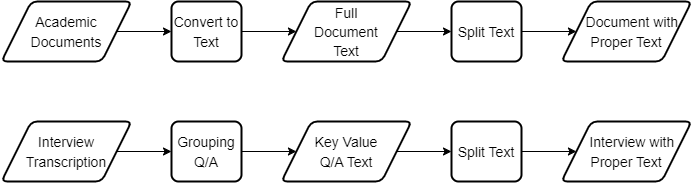
\includegraphics[scale=0.4]{eng-preproc.png}}
        \caption{Data Preprocessing}
        \label{fig:preprocessing}
    \end{figure}
    
\begin{enumerate}
    \item \textbf{Pre-Processing Document Data} \\
    Initially, data from academic documents, typically in PDF format, undergoes conversion from PDF to text using the Langchain framework\'s document loader. Specifically, we use the \textbf{PyPDFLoader} from \textbf{document\_loaders} in Langchain to perform this conversion. This step ensures that the text is in a format that can be processed by the LLM. After conversion, the text from the documents is segmented by sentences, enabling the LLMs to understand the content more deeply by considering sentence structure. This segmentation is crucial to ensure that information from the documents can be effectively accessed and comprehended by the model.
    
    \item \textbf{Pre-Processing Interview Data} \\
    For interview data, automatic transcription is performed using the \textbf{YouTubeLoader} library from Langchain\'s  \textbf{document\_loaders}. This library facilitates the automatic extraction and transcription of audio from interviews. The initial step involves grouping questions and answers into related entities, allowing the model to comprehensively understand the context of the discussions. Following this, the pre-processing of interview data mirrors that of document data, with text segmentation by sentences. This creates a uniform data structure, facilitating the model\'s understanding of information extracted from interviews.
\end{enumerate}

Through meticulous and careful pre-processing, the data is expected to provide a better and more contextual representation when presented to the LLMs. This process serves as a crucial initial step in building a reliable and effective KAS in the academic environment.

\subsection{LLM}
The next stage after data pre-processing is knowledge extraction using the LLMs. The LLMs process is illustrated in Figure \ref{fig:llm}.

\begin{figure}[htbp]
    \centerline{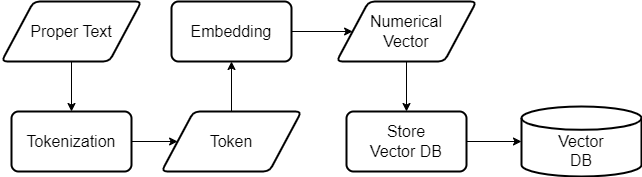
\includegraphics[scale=0.4]{eng-llm.png}}
    \caption{LLMs Process}
    \label{fig:llm}
\end{figure}

This process includes several critical steps outlined as follows:

\begin{enumerate}  
    \item \textbf{Tokenization} \\
    After reading the text, tokenization is performed to break the text into tokens or smaller units that can be processed by the model. Tokenization helps the model to understand the structure and meaning of words within the context of sentences.
    
    \item \textbf{Embedding} \\
    The embedding process involves representing words as numerical vectors. Each word in the text is transformed into a vector that captures the word's meaning. This process allows the model to work with continuous representations and to understand semantic relationships between words.
    
    \item \textbf{Storing in Vector Database} \\
    The vectors generated from the embedding process are stored in a Vector Database (Vector DB). The Vector DB acts as a repository for the vector representations of the processed documents and interviews. This stored data serves as the knowledge base that can be accessed in subsequent stages.
\end{enumerate}

By using the LLMs, the system can understand and represent the information extracted from documents and interviews more effectively. These steps connect the understanding of text with vector representations that the system can access and process in later stages.

\subsection{Fine Tuning}
Fine-tuning is a critical stage in optimizing the model to respond more accurately and relevantly to specific questions or contexts. We divided the fine tuning into two subprocesses: first at the individual level using a single Vector Database (Vector DB), and second at the aggregation level using a combined vector database.

\begin{enumerate}
    \item \textbf{Fine Tuning \#1} \\
        Figure \ref{fig:fine-tuning-1} illustrates the process of the first fine-tuning phase. This phase begins with the use of a single Vector Database as input. Each vector from the Vector DB is involved in the fine-tuning process to enhance the model's ability to understand the content and respond more accurately. Fine-tuning is achieved through the use of Neural Network layers, which in this context are equivalent to embeddings. The goal of this phase is to produce vector representations that are more contextual and relevant to the individual information sources. The term "contextual" here means that the vector store saves these embeddings in a way that captures multiple meanings or synonyms, derived from GPT, allowing the model to better understand the nuances and context of the information.

        \begin{figure}[htbp]
            \centerline{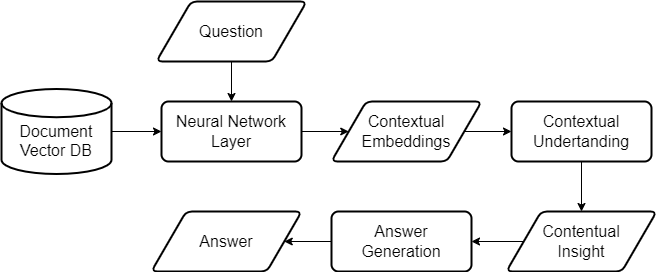
\includegraphics[scale=0.4]{eng-fine1.png}}
            \caption{Fine Tuning}
            \label{fig:fine-tuning-1}
        \end{figure}

        Following fine-tuning, the model undergoes a stage of \textbf{Contextual Understanding}.  At this stage, the model uses GPT to consider the context more comprehensively, allowing for better interpretation of user questions or inputs. This process integrates contextual understanding, meaning the model is capable of recognizing similar text or synonyms, ensuring that responses are aligned with the given context even when different wording is used.

        The final step of the first fine-tuning phase is \textbf{Answer Generation}. In this phase, the optimized model generates answer based on the contextual understanding and enhanced vector representations. This involves similarity search to match user queries with the most relevant information from the database and generate an appropriate response.
                    
    \item \textbf{Fine Tuning \#2} \\
        The second fine-tuning phase, involves a similar process but at the aggregation level using the combined vector database. In this stage, vector representations from various sources of information are integrated, and the model undergoes another round of fine-tuning. The focus here is on understanding and responding to questions or contexts that involve multiple aspects of knowledge acquisition.
\end{enumerate}

            
The process for the fine-tuning phase includes:
\begin{itemize}
    \item Input: Vector database and user questions.
    \item Neural Layer: Embeddings representing the integrated vectors.
    \item Contextual Understanding: Using GPT for a comprehensive understanding of the context to create Contextual Insights.
    \item Answer Generation: Performing similarity search to generate a answer based on the  knowledge.
\end{itemize}

Through these two stages of fine-tuning, it is anticipated that the model will deliver improved knowledge acquisition results, taking into account the depth of information from the involved sources and generating more contextual and relevant responses.


\section{System Demonstration and Practical Use}
\subsection{Tools and Technologies Used}
The development and functionality of the system are powered by several key technologies:
\begin{itemize}
    \item Streamlit: Used for the front-end interface of the web-based chatbot, enabling users to interact with the system in a user-friendly manner.
    \item Langchain: A critical framework used to integrate different language models, such as GPT, and manage workflows for document processing and question answering.
    \item FAISS Vector Store: Used for storing and retrieving vectorized embeddings of the knowledge processed from the input data. This ensures efficient and accurate search capabilities within the knowledge base.
    \item OpenAI Embedding and Chat: The core LLMs and embedding generation tool. OpenAI's GPT is used to generate embeddings, process user inputs, and provide accurate, context-based responses.
\end{itemize}

\subsection{Input Page: Data Upload and Processing}
This section of the system allows users to upload various types of data to be processed and added to the knowledge base. Users can submit different data formats to capture knowledge in diverse ways:
\begin{itemize}
    \item PDF Files: Users can upload academic documents, research papers, or administrative files, which are processed using Langchain's PyPDFLoader. The system extracts the text and converts it into a structured format.
    \item JSON Files: Structured data in JSON format can be directly uploaded, allowing the system to quickly process datasets or academic records.
    \item YouTube URLs: Leveraging Langchain's YouTubeLoader, users can input a YouTube URL for automatic transcription. The system extracts the text from the video’s captions and processes it for further use.
    \item Raw Text: Users can input plain text directly, making the system flexible for adding knowledge from various informal sources like interviews, lectures, or meeting notes.
\end{itemize}

Once the input data is uploaded, the system processes and converts it into embeddings using OpenAI’s embedding model. The vectorized data is stored in the FAISS Vector Store for quick and contextually relevant retrieval.

\subsection{Chatbot Page: Interactive Knowledge Access}
The chatbot interface allows users to interact directly with the knowledge stored in the system:
\begin{itemize}
    \item \textbf{Interaction with Knowledge}: Users can ask questions related to the data that has been processed and stored in the vector database. The chatbot leverages GPT to understand the questions, retrieve relevant information from the embeddings, and generate contextual answers.
    \item \textbf{Memory Scenario}: The chatbot incorporates a memory scenario where session-specific data is stored temporarily. This allows the chatbot to maintain a context-aware conversation within a session, enabling it to remember past questions and answers. However, this session memory is cleared once the session ends, ensuring privacy and a fresh start for future interactions.
\end{itemize}

For example: \\
\textbf{User's Question}: \textit{``What should be considered in the Final Project revision process?''} \\

\textbf{Chatbot Response}: \\
In the Final Project revision process, the following points must be considered:
\begin{enumerate}
    \item Students are given a maximum of 15 calendar days to complete the revision after the results of the Final Project hearing are decided.
    \item If the revision is not completed within 15 days, the Final Project index value will drop by one level.
    \item If the revision is not completed within 30 days, the student is declared to have failed.
    \item The results of the revision must be validated by the Supervisor before being submitted to the LAAK admin for the Judicial Hearing process.
\end{enumerate}


\section{Evaluation}
To obtain a comprehensive and optimal evaluation of the KAS, we use three primary evaluation metrics: ROUGE Score, BERTScore, and manual evaluation. Combining these three methods allows for a thorough assessment of the quality of answers generated by the system.

\subsection{ROUGE Score}
ROUGE Score (Recall-Oriented Understudy for Gisting Evaluation) measures the similarity between the generated summaries and reference texts by calculating precision, recall, and F1 score based on n-gram overlap. This metric provides insight into the surface-level text similarity, such as words and phrases, between the generated summaries and reference texts \cite{Lin2004}. It helps assess how well the generated summaries match the reference texts considered as gold standard.
\begin{itemize}
    \item \textbf{Precision}: Precision is calculated using the formula:
    \[
    \text{Precision (P)} = \frac{\text{TP}}{\text{TP + FP}}
    \]
    where:
    \begin{itemize}
        \item TP (True Positives): The number of overlapping n-grams between the generated results and the reference. In the context of ROUGE-N, this includes n-grams appearing in both the generated result and the reference text.
        \item TP+FP (Total Predicted Positives): The total number of n-grams in the generated results. This includes both correctly and incorrectly predicted n-grams.
    \end{itemize}
    A higher precision value indicates that the generated results are more accurate and aligned with the reference content.

    \item \textbf{Recall}: Recall is calculated using the formula:
    \[
    \text{Recall (R)} = \frac{\text{TP}}{\text{TP + FN}}
    \]
    where:
    \begin{itemize}
        \item TP (True Positives): The number of overlapping n-grams between the generated results and the reference.
        \item TP+FN (Total Actual Positives): The total number of n-grams in the reference text. This includes all n-grams that should have been generated based on the reference.
    \end{itemize}
    Recall provides insight into how well the predictions capture the information present in the reference. A high recall value indicates that the predictions cover most of the relevant information from the reference.

    \item \textbf{\( F_{1}\text{-score} \)}: 
    \( F_{1}\text{-score} \) is calculated using the formula:
    \[
    F_{1}\text{-score} = 2 \times \left( \frac{\text{Precision} \times \text{Recall}}{\text{Precision} + \text{Recall}} \right)
    \]
    \( F_{1}\text{-score} \) combines precision and recall into a single metric that provides a holistic view of the summary quality. A higher \( F_{1}\text{-score} \) indicates a better balance between precision and recall.
\end{itemize}
    
\subsection{BERTScore}
BERTScore evaluates semantic similarity between the generated text and reference text using contextual embeddings from the BERT model \cite{Zhang2020}. BERTScore calculates precision, recall, and F1 score based on deeper semantic understanding, offering a better assessment of answer quality in terms of relevance and contextual alignment compared to traditional n-gram metrics.
\begin{itemize}
    \item \textbf{Precision}: Precision is calculated using the formula:
    \[
    \text{Precision} (P) = \frac{1}{|G|} \sum_{w \in G} \max_{w' \in R} \text{sim}(w, w')
    \]
    where:
    \begin{itemize}
      \item \( G \) is the set of words in the generated text.
      \item \( R \) is the set of words in the reference text.
      \item \( \text{sim}(w, w') \) is the cosine similarity between the embeddings of words \( w \) and \( w' \).
    \end{itemize}

    \item \textbf{Recall}: Recall is calculated using the formula:
    \[
    \text{Recall} (R) = \frac{1}{|R|} \sum_{w \in R} \max_{w' \in G} \text{sim}(w, w')
    \]
    where:
    \begin{itemize}
      \item \( R \) is the set of words in the reference text.
      \item \( G \) is the set of words in the generated text.
      \item \( \text{sim}(w, w') \) is the cosine similarity between the embeddings of words \( w \) and \( w' \).
    \end{itemize}

    \item \textbf{\( F_{1}\text{-score} \)}: 
    \( F_{1}\text{-score} \) is calculated using the formula:
    \[
    F_{1}\text{-score} = 2 \times \left( \frac{\text{Precision} \times \text{Recall}}{\text{Precision} + \text{Recall}} \right)
    \]
\end{itemize}
    
\subsection{Manual Evaluation}
Manual evaluation involves experts providing direct feedback on the accuracy and relevance of the answers generated by the system. Experts assess answers based on criteria such as factual accuracy, completeness of information, and contextual appropriateness. This evaluation method provides deeper insights into the quality of answers that cannot be captured by automatic metrics alone, such as ROUGE Score and BERTScore.


For this study, we employed two experts with over 25 years of experience in their respective fields, including a program secretary who is deeply familiar with academic processes and tacit knowledge within the institution. Their expertise was crucial in evaluating the system’s performance, ensuring that the generated answers were both practically applicable and aligned with institutional standards.

To evaluate the system, we posed questions across 6 distinct topics, with 10 questions per topic. Each answer was assessed for relevance on a scale ranging from "not relevant" to "highly relevant." This approach allowed us to measure how well the system addressed the questions within each topic and provided comprehensive insights into the system’s ability to generate contextually appropriate and accurate responses.

\subsection{Results}
Combining these three approaches ensures a comprehensive assessment of the KAS, considering both surface-level text similarity and semantic similarity, and provides a fuller picture of the quality of the answers produced by the system.

For more detailed information, the model performance results with ROUGE Score can be seen in Table\ref{tab:rouge-table}. The table shows that scoring using unigrams dominates, with precision as the highest metric.

\begin{table}[htbp]
    \centering
    \caption{Rouge Score}
    \setlength{\arrayrulewidth}{0.5pt} % Adjust the thickness of vertical lines
    \renewcommand{\arraystretch}{1.5} % Adjust vertical spacing
    \begin{tabular}{|c|c|c|c|c|c|c|}
        \cline{2-7}
        \multicolumn{1}{c|}{} & \multicolumn{3}{c|}{\textbf{Unigram}} & \multicolumn{3}{c|}{\textbf{Bigram}} \\ 
        \hline
        \textbf{Dataset} & \textbf{PREC} & \textbf{REC} & \textbf{F1} & \textbf{PREC} & \textbf{REC} & \textbf{F1} \\
        \hline
        Document & \textbf{0.72} & 0.12 & 0.20 & 0.38 & 0.04 & 0.09 \\ 
        \hline
        Interview & \textbf{0.79} & 0.11 & 0.19 & 0.40 & 0.03 & 0.06 \\ 
        \hline
        Combined & \textbf{0.74} & 0.13 & 0.21 & 0.40 & 0.05 & 0.09 \\ 
        \hline
    \end{tabular}
    \label{tab:rouge-table}
\end{table}

\begin{table}[htbp]
    \centering
    \caption{BERT Score}
    \setlength{\arrayrulewidth}{0.5pt} % Adjust the thickness of vertical lines
    \renewcommand{\arraystretch}{1.5} % Adjust vertical spacing
    \begin{tabular}{|c|c|c|c|}
        \cline{2-4}
        \hline
        \textbf{Dataset} & \textbf{PREC} & \textbf{REC} & \textbf{F1}  \\
        \hline
        Document & \textbf{0.74} & 0.58 & 0.65 \\ 
        \hline
        Interview & \textbf{0.76} & 0.60 & 0.67 \\ 
        \hline
        Combined & \textbf{0.75} & 0.59 & 0.66 \\ 
        \hline
    \end{tabular}
    \label{tab:bert-table}
\end{table}

For the model performance results with BERTScore can be seen in Table \ref{tab:bert-table}. The table shows that the model performs well contextually, with the highest score still obtained in the precision metric. A high precision score indicates that the model tends to produce answers that are highly relevant and semantically in line with the existing references.

However, the combined dataset scored lower than the interview dataset due to the PDF-to-text extraction in documents. This extraction method has weaknesses that affect the quality of the text, leading to a lower combined result. Therefore, even though the precision score is high, it is important to consider recall and F1 score metrics. A lower recall score may indicate that the model missed some relevant information, and the F1 score balances precision and recall, highlighting areas for improvement.

Then, for the manual evaluation results, the evaluators were two individuals who provided the tacit knowledge for the system: an academic secretary and a senior lecturer. Their role was crucial as they had firsthand experience with the implicit knowledge encoded into the system, enabling them to assess the relevance of the system's responses accurately.

The evaluation results are as follows:the following results were obtained: \\
Out of a total of 60 questions:
\begin{itemize}
    \item \textbf{86}\% of the answers were rated as \textbf{highly relevant} with a score of 3.5 - 5
    \item \textbf{2}\% of the answers were rated \textbf{moderately relevant} with a score of 3
    \item and only \textbf{12}\% of the answers were rated \textbf{less relevant} with a score of 1-2.5
\end{itemize}

These results show that the system performs quite well in answering questions in a relevant and contextual manner according to expert judgment.

Thus, the use of the ROUGE metric as a guide for quantitative evaluation, then the BERT metric for semantic evaluation and together with the input from the expert evaluation, can provide a more holistic and detailed understanding of the overall quality of the developed text generation system.

\section{Conclusion}
\subsection{Conclusion}
In this research, a system for automatic knowledge acquisition in the academic domain has been successfully proposed and implemented using LLMs and fine-tuning techniques. The evaluation conducted shows that the system is capable of acquiring, understanding, and responding to various types of questions and contexts related to the academic environment.

The precision of knowledge acquisition, measured by comparison with information provided by experts in interviews, demonstrates positive results. The responses generated by the system also show a good level of contextuality, with the ability to respond accurately to questions referring to information from academic documents and interview results.

However, there are areas that can be improved. Analyzing the system's speed and efficiency could be a focus for further development to ensure responsiveness in a dynamic academic environment.

Overall, the system has shown good precision, particularly in tests using questions that align with the existing documents. However, to further enhance performance, improvements in both data and system development are needed. Thus, these improvement steps will be an integral part of future development to ensure the success and reliability of the KAS in the academic environment.


%
% ---- Bibliography ----
%
% BibTeX users should specify bibliography style 'splncs04'.
% References will then be sorted and formatted in the correct style.
%
\bibliographystyle{splncs04}
\bibliography{references}
%
\end{document}
